\documentclass[a4paper, 12pt]{article}
\usepackage{graphicx}
\usepackage{hyperref}
\usepackage{float}
\usepackage{caption}
\usepackage{listings}
\usepackage{qrcode}


\title{\textbf{Automatic Door Lock}}
\author{Team 11 \\ 2024112001 Kshitij Patkar \\ 2024112005 Harry Jain \\ TA \\ S S Ananya Varma Ganapathiraju}
\date{2nd December, 2024}

\begin{document}
\maketitle
\tableofcontents
\newpage

\section{Problem Statement}
In today's world, security is of utmost importance. Traditional door-locking mechanisms are becoming increasingly inadequate due to their susceptibility to tampering and lack of interactive features. There is a growing need for an innovative and technologically advanced solution that provides secure, user-friendly, and efficient access control. This project addresses this need by developing a \textbf{Secure and Interactive Door Locking System}, designed to ensure robust access management with modern, interactive features.

\subsection*{Objective}
The objective of this project is to develop a secure and interactive door-locking system utilizing a password-based entry mechanism. The system will incorporate real-time feedback, enhanced security measures, and convenient management options, ensuring a modern approach to access control.

\subsection*{Key Features Addressed}
\begin{enumerate}
    \item \textbf{Password-Based Entry with Real-Time Feedback:}
    \begin{itemize}
        \item Password authentication mechanism for secure entry.
        \item LCD display providing real-time feedback, such as \textit{"Correct"} or \textit{"Incorrect"}.
        \item A buzzer system to provide auditory alerts for successful entries and failed attempts.
    \end{itemize}
    
    \item \textbf{Lockout Mechanism to Prevent Unauthorized Access:}
    \begin{itemize}
        \item Mechanism to lock the system temporarily after repeated failed password attempts.
        \item Prevents unauthorized access through brute-force attacks.
    \end{itemize}
    
    \item \textbf{Password Customization and Secure Management Options:}
    \begin{itemize}
        \item Users can set, update, and manage passwords securely.
        \item User-friendly interface for password customization.
    \end{itemize}
    
    \item \textbf{Integration with a Bluetooth-Enabled App:}
    \begin{itemize}
        \item Remote control of the locking system via a Bluetooth-enabled application.
        \item Enhanced convenience for managing access.
    \end{itemize}
\end{enumerate}

\subsection*{Conclusion}
This project aims to design and implement a secure, interactive, and modern door-locking system that caters to the growing need for advanced access control. By integrating password-based entry, real-time feedback, robust security mechanisms, and app-based remote control, this system provides a comprehensive solution for both residential and commercial applications.


\section{Aim of the Project}
The aim of this project is to design and implement a robust, automated door-locking system utilizing Arduino. The system is intended to provide a secure and convenient solution for access control by integrating multiple modern features, including:

\begin{itemize}
    \item \textbf{Keypad-Based Entry:} 
    A user-friendly membrane keypad is implemented for password entry, allowing users to securely unlock the door using a personalized passcode.
    
    \item \textbf{Remote Control via Bluetooth Module:} 
    The system incorporates a Bluetooth module to enable remote access control. This feature allows users to unlock or manage the system conveniently through a smartphone application, ensuring flexibility and enhanced convenience.
    
    \item \textbf{Visual Feedback Through LCD Display:} 
    An LCD display is included to provide real-time visual feedback during system operations. It displays messages such as \textit{"Enter Password," "Correct," "Incorrect,"} or \textit{"Too many incorrect attempts"} to enhance user interaction and provide clear, intuitive guidance.
    
    \item \textbf{Enhanced Security Mechanisms:}
    To prevent unauthorized access, the system incorporates features such as a temporary lockout after repeated incorrect password attempts, reducing the risk of brute-force attacks.
    
    \item \textbf{Solenoid Lock for Improved Reliability:} 
    The system employs a solenoid lock instead of a servo motor paired with a mechanical lock. This choice eliminates the need to deal with physical variables like friction and large moving parts, which can compromise reliability and introduce additional wear and tear. A solenoid lock provides a more elegant and efficient solution, ensuring smoother operation and improved durability for a modern, compact, and maintenance-friendly design.
\end{itemize}

The project aims to deliver a highly secure and interactive door-locking solution suitable for modern access control needs in residential, commercial, and industrial environments. The integration of automated features, real-time feedback, and remote control capabilities ensures an effective, user-friendly, and technologically advanced security system.


\section*{Components Used}
The following components were carefully selected and integrated to develop a secure, interactive, and efficient automated door-locking system:

\begin{itemize}
    \item \textbf{Arduino Uno:} 
    The core microcontroller used to handle all inputs, process logic, and control outputs. Powered by a power bank, the Arduino Uno ensures portability and uninterrupted operation.

    \item \textbf{12V Solenoid Door Lock with Relay Module:} 
    A solenoid door lock, controlled via a relay module, serves as the main locking mechanism. Unlike servo motors paired with mechanical locks, the solenoid lock provides a more elegant and robust solution by eliminating mechanical issues such as friction, wear and tear, and large moving parts. It offers smoother operation and improved reliability, making it an ideal choice for modern access control.

    \item \textbf{16x2 LCD Screen with I2C Module:} 
    A 16x2 LCD screen equipped with an I2C module is used for real-time feedback and status display. Messages such as \textit{"Enter Password," "Correct," "Incorrect,"} or \textit{"Too many incorrect attempts"} are displayed to guide the user and enhance system interaction. The I2C module simplifies wiring and reduces the number of pins required.

    \item \textbf{3x4 Membrane Keypad:} 
    A compact, user-friendly keypad is implemented for password input. It allows users to securely enter a passcode, ensuring an intuitive and accessible interface for accessing the locking system.

    \item \textbf{Buzzer:} 
    A buzzer is included for audible feedback and alerts. It generates beeping sounds for specific actions such as successful unlocking, denied access, or system lockouts due to repeated failed attempts.

    \item \textbf{Bluetooth Module:} 
    A Bluetooth module is integrated for remote control of the locking system. This module pairs with a mobile application created using the MIT App Inventor, allowing users to manage the lock wirelessly and providing an added layer of convenience.

    \item \textbf{Custom PCB Board:} 
    A custom-designed and hand-soldered circuit board (PCB) is used to solder and organize all the electronic components neatly. This ensures a more compact and reliable setup compared to using breadboards or loose wiring.

    \item \textbf{Cardboard Box:} 
    A cardboard enclosure is used to house and protect all components. This makes the system portable and provides a functional prototype housing for demonstration purposes.

\end{itemize}

Each component plays a critical role in ensuring the system's functionality, reliability, and user-friendliness, contributing to an advanced and effective automated door-locking solution.


\section{Circuit Schematics and Process Diagrams}
\begin{figure}[H]
    \centering
    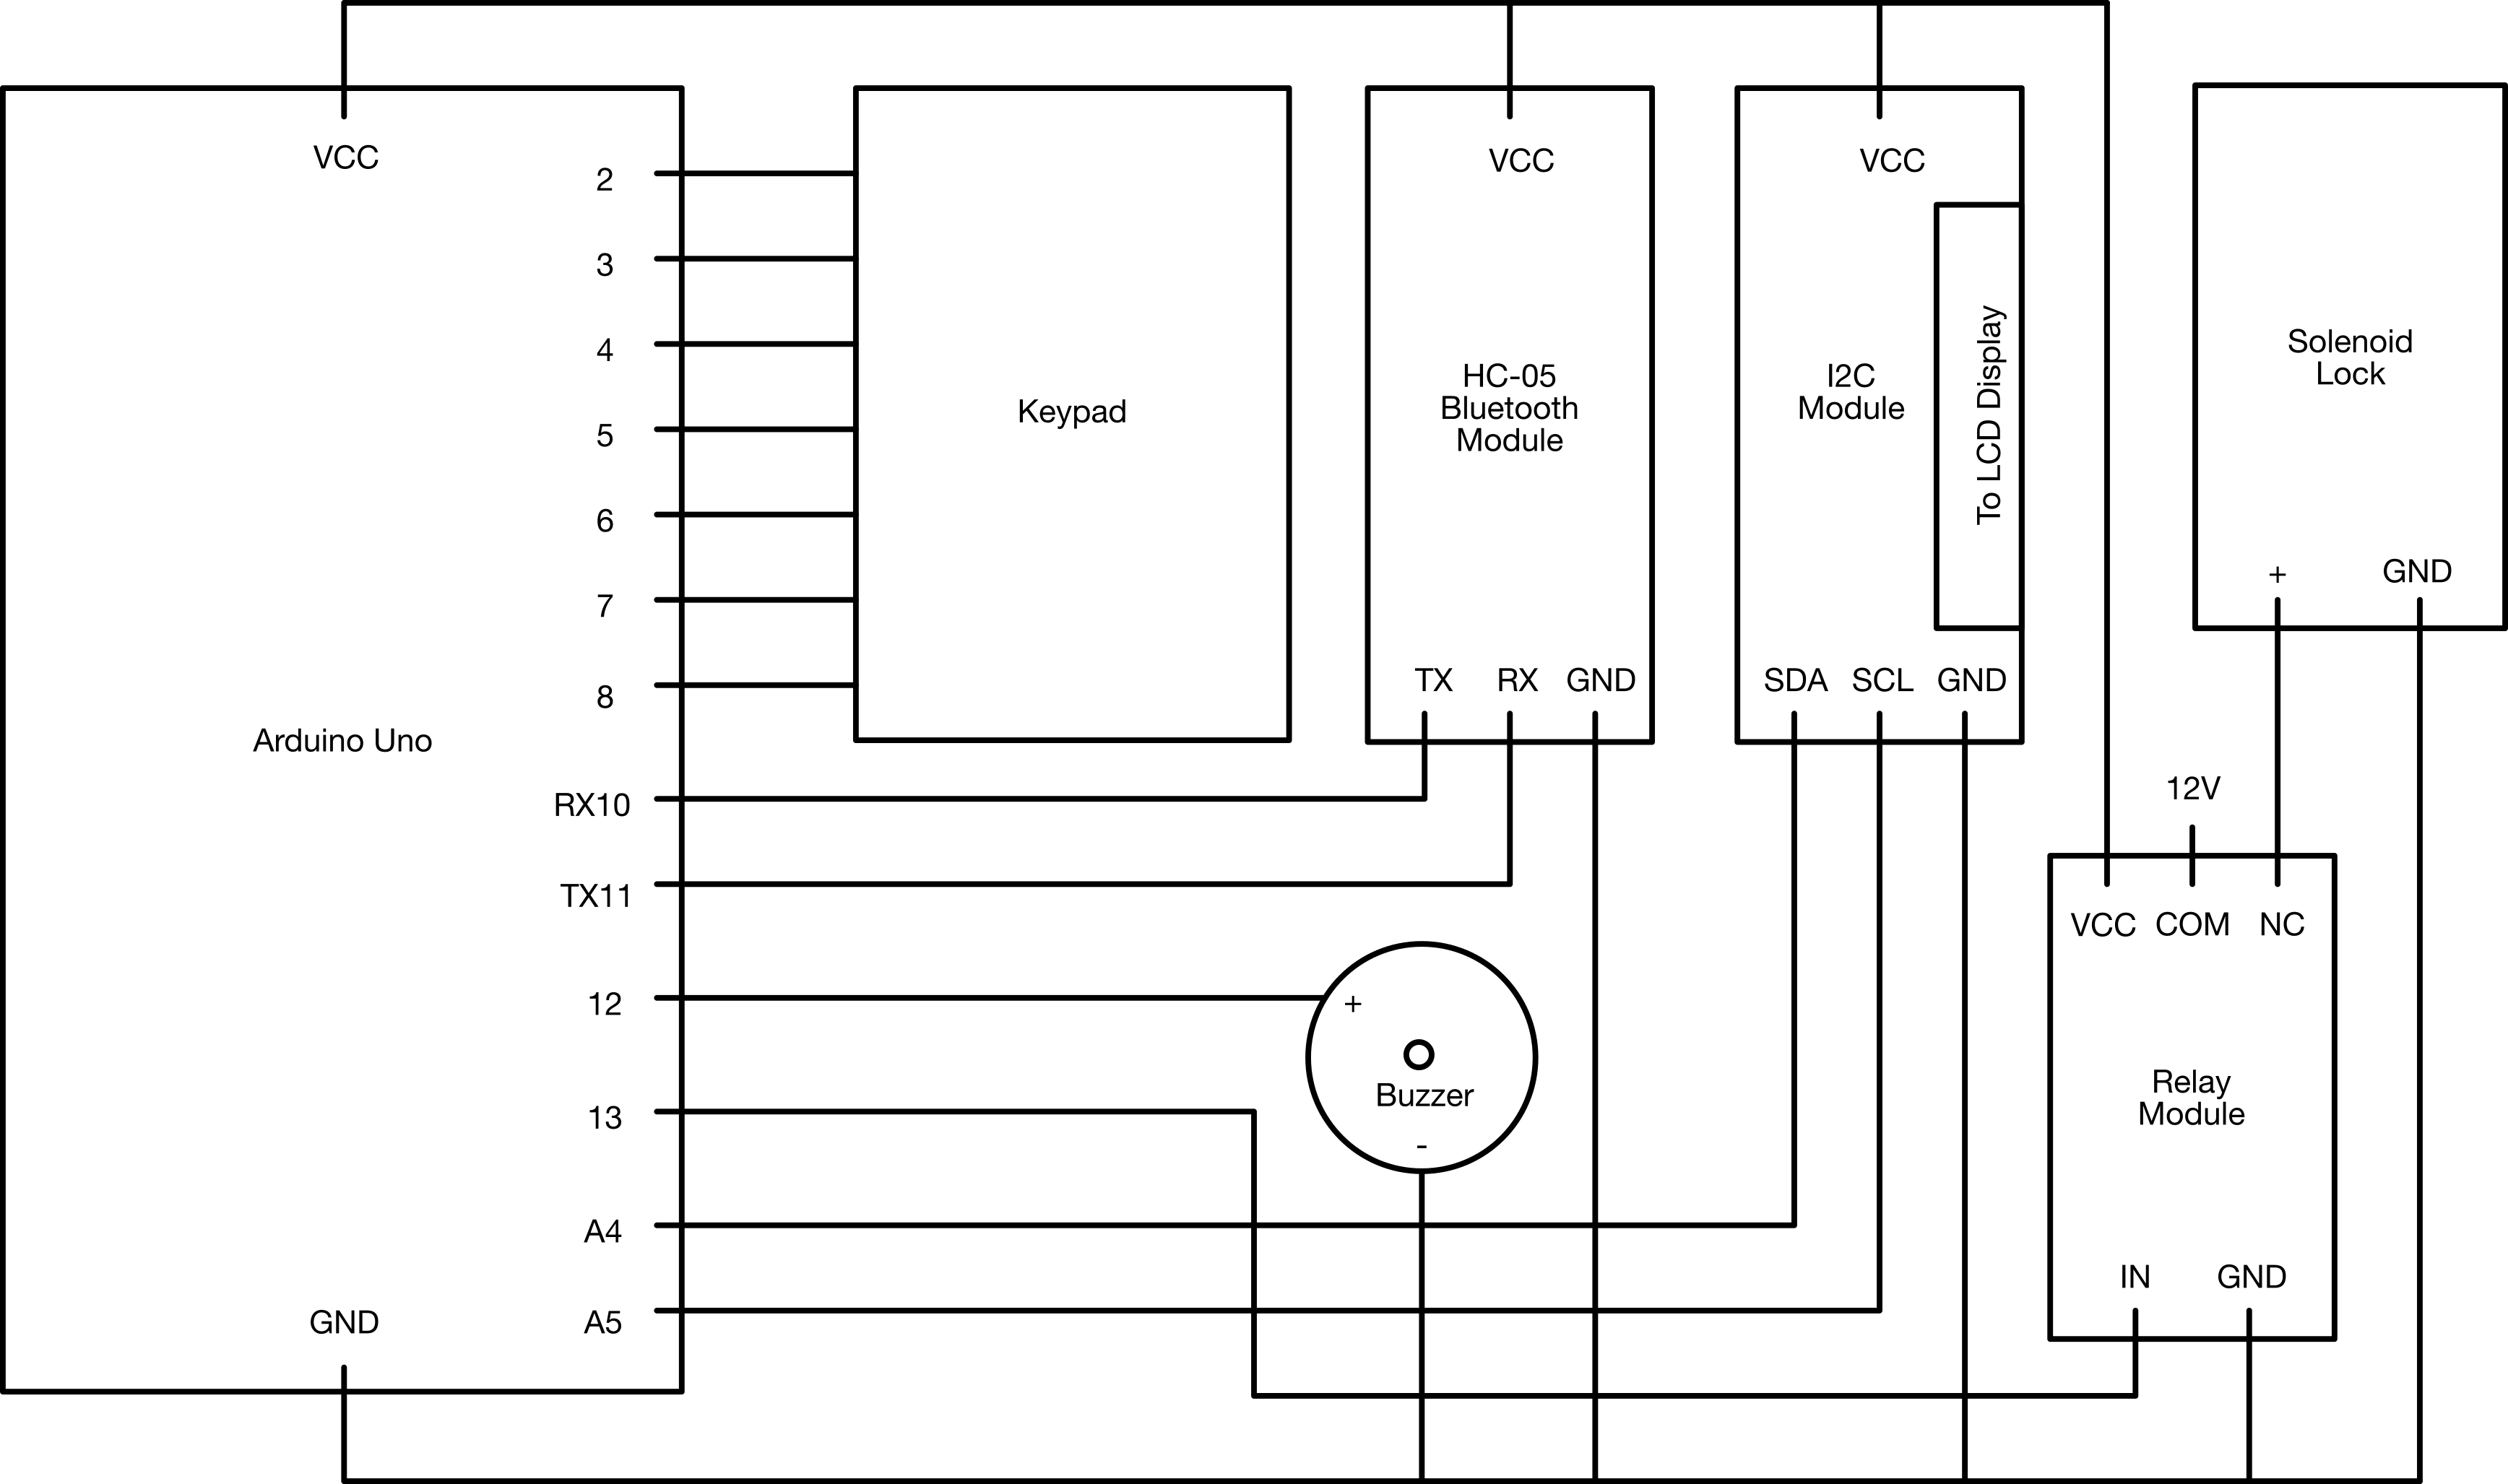
\includegraphics[width=0.8\textwidth]{circuit.png}
    \caption{Circuit Schematic}
\end{figure}

\begin{figure}[H]
    \centering
    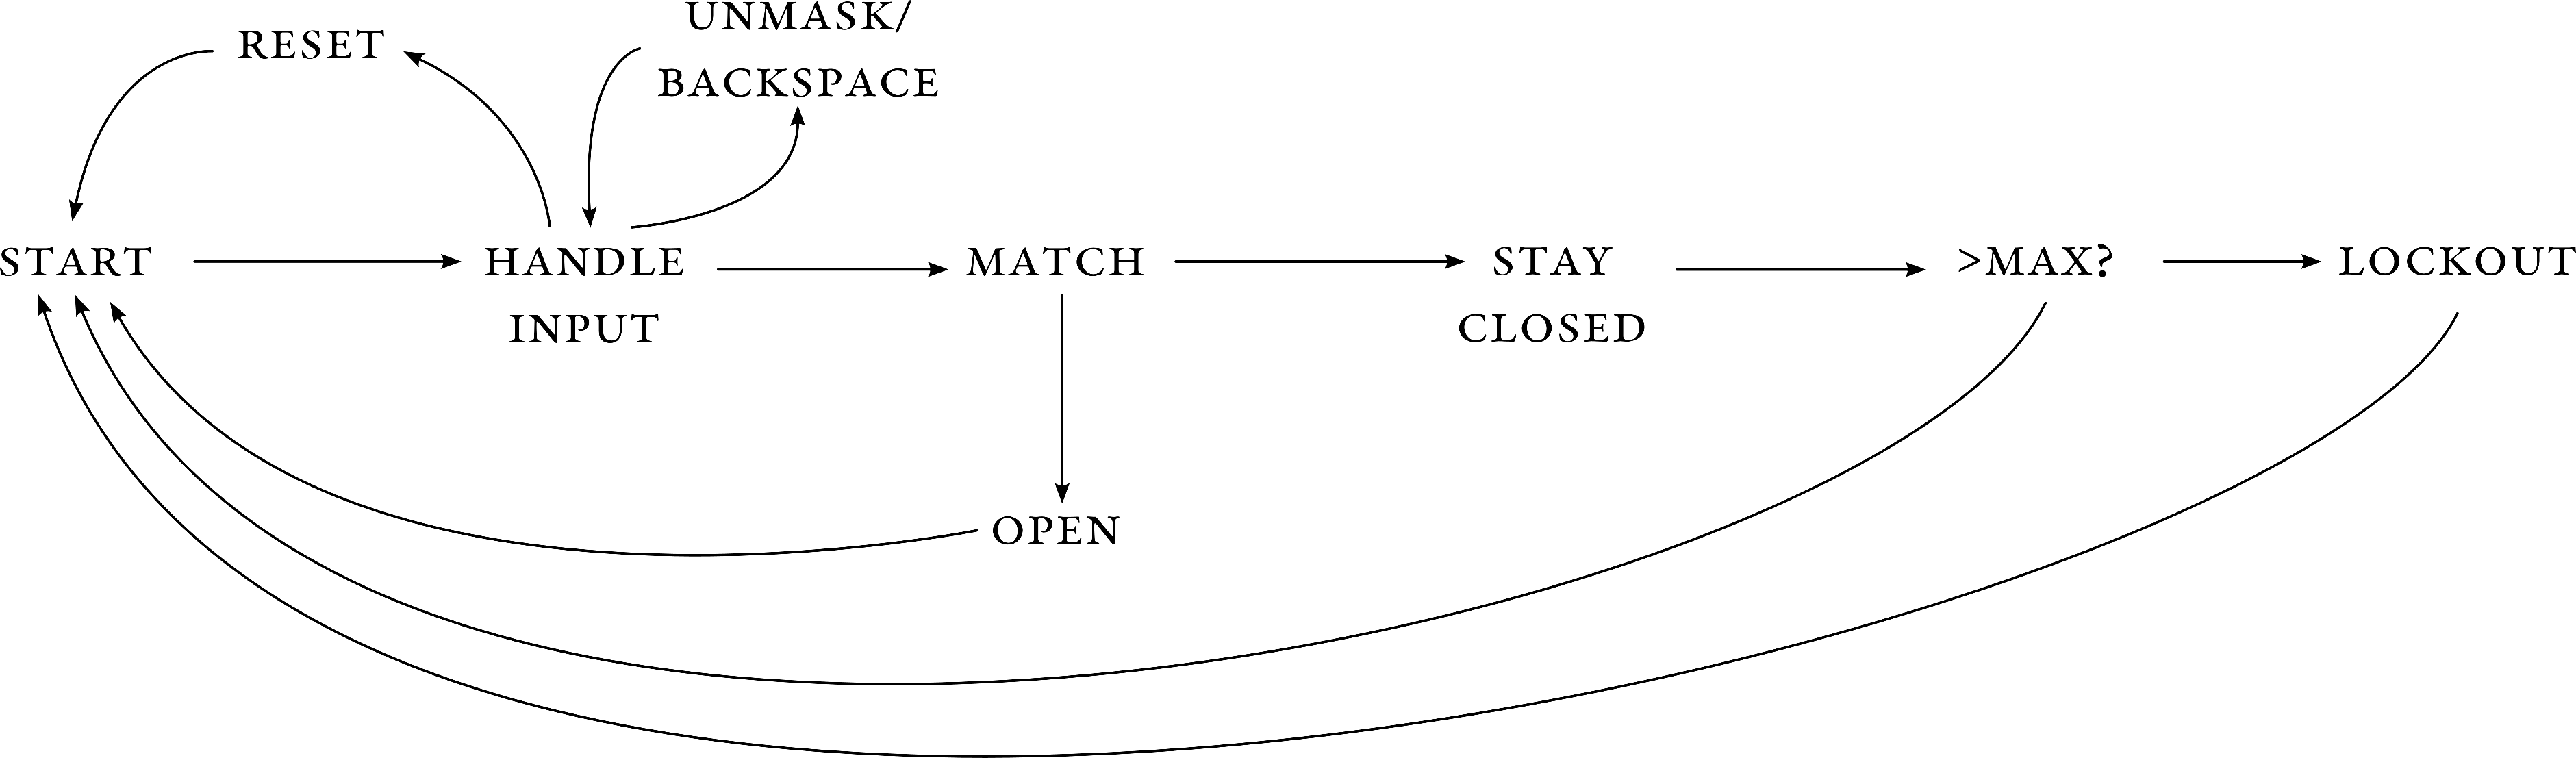
\includegraphics[width=0.8\textwidth]{process.png}
    \caption{Process Diagram}
\end{figure}

\section{Flowchart}
\begin{figure}[H]
    \centering
    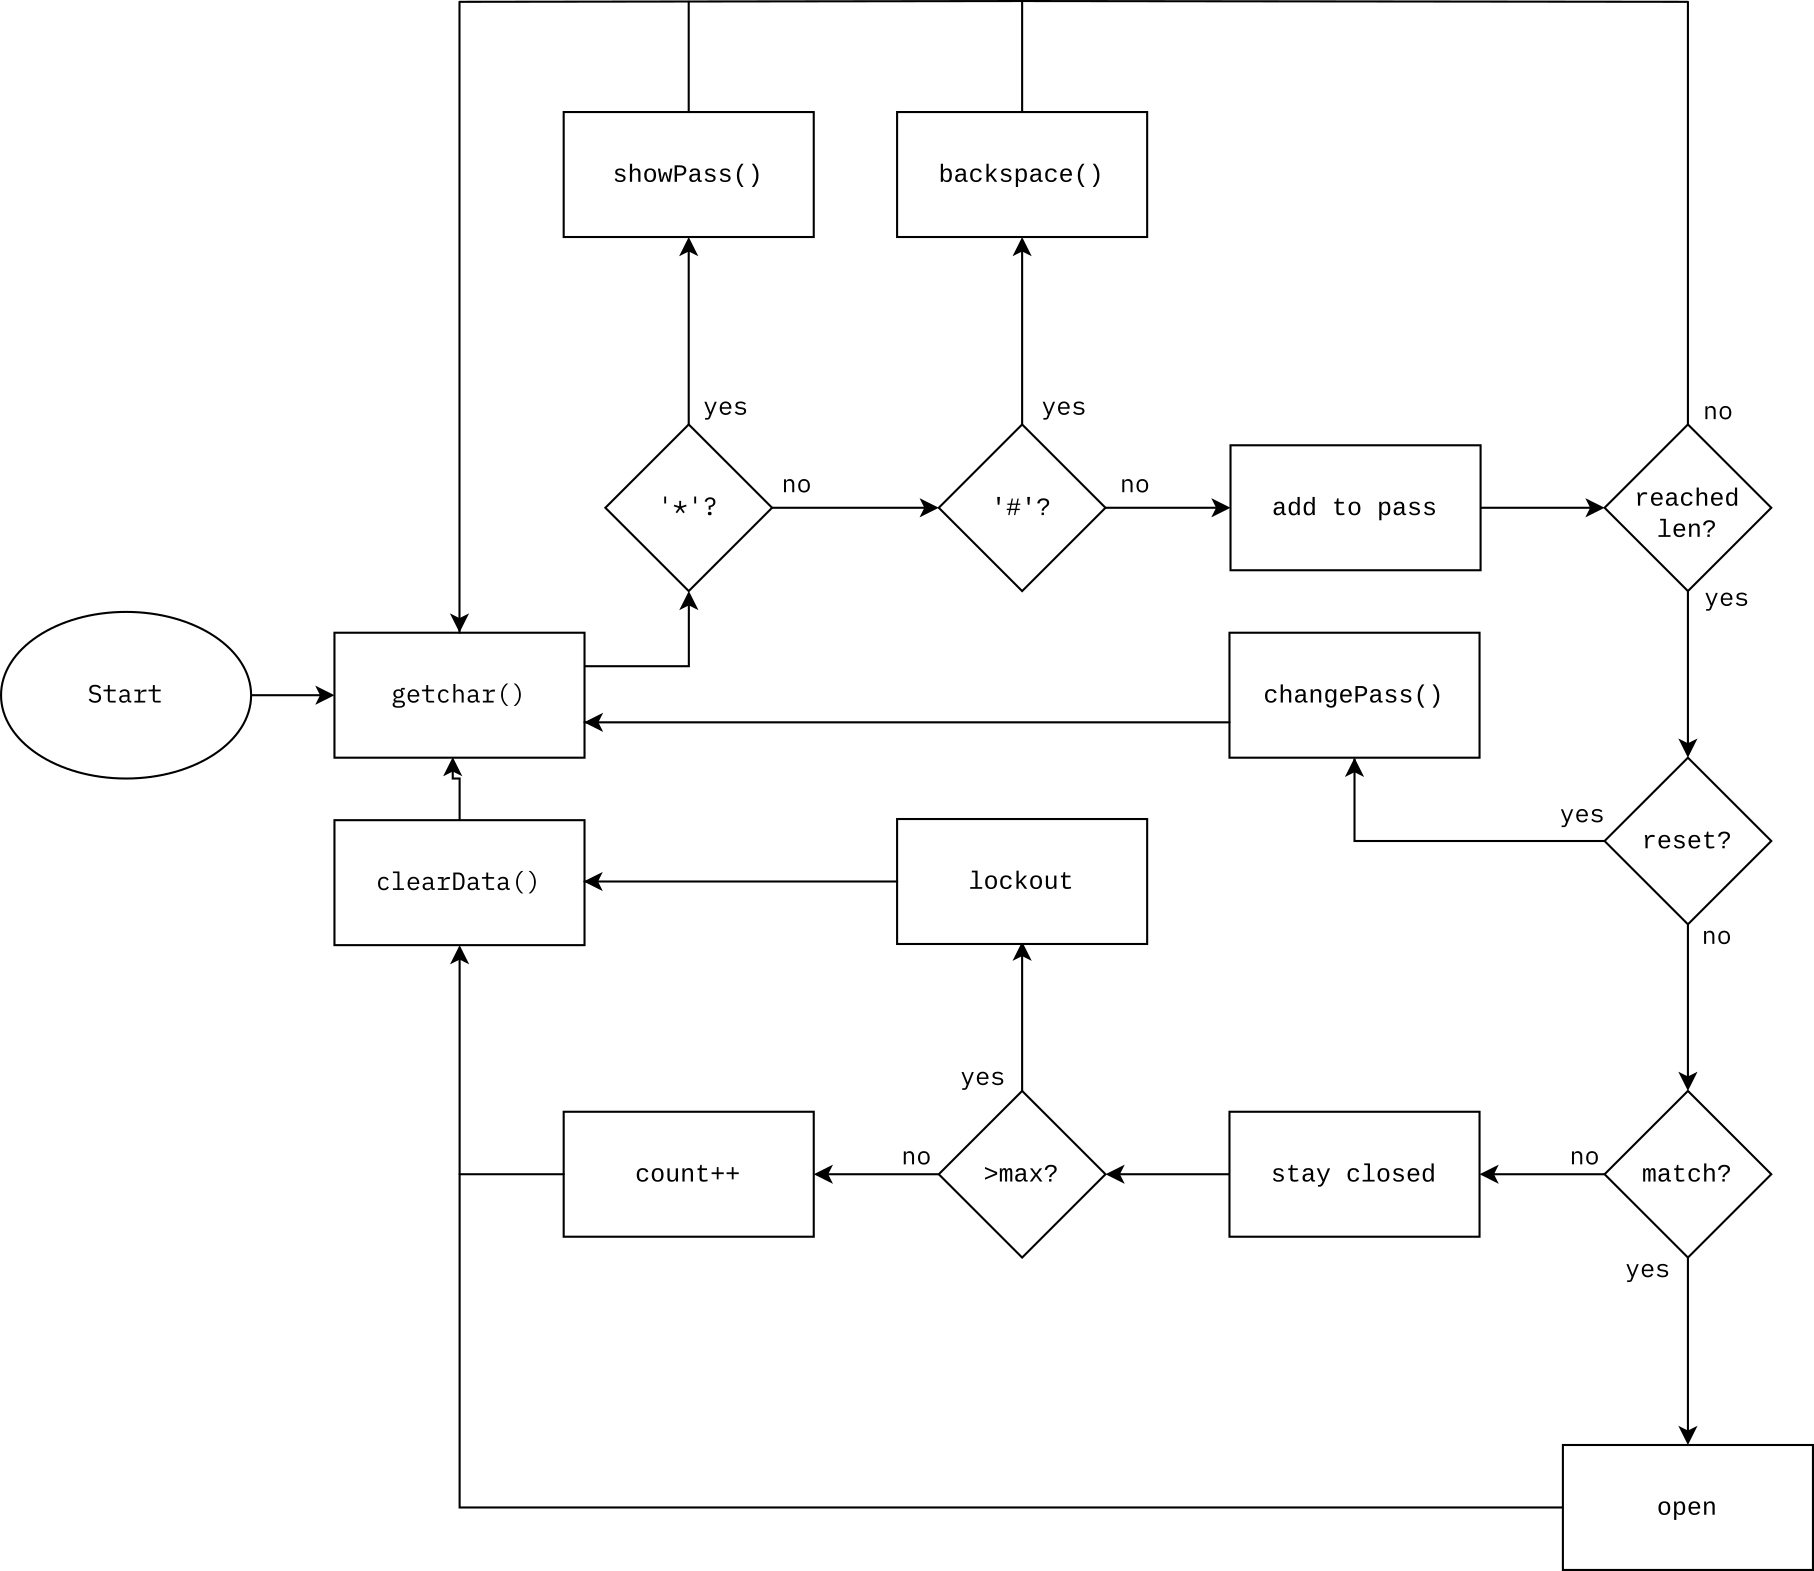
\includegraphics[width=0.8\textwidth]{flowlight.png} 
    \caption{Flowchart}
\end{figure}

\section*{Description of the Project}

The Automatic Door Lock project is an innovative solution designed to enhance the security and convenience of access control systems. Built around an Arduino Uno microcontroller, this system integrates a range of hardware and software features to ensure ease of use, reliability, and robustness. Below is a comprehensive breakdown of the key functionalities and features of the project:

\begin{itemize}
    \item \textbf{Password Input:} 
    The system employs a 3x4 membrane keypad for secure password entry. This keypad is compact, durable, and provides tactile feedback, making it an ideal choice for user-friendly interaction. Users can enter passwords with ease, which are processed by the Arduino Uno for verification. The keypad also supports the following special inputs:
    \begin{itemize}
        \item \textbf{* (Unmasking):} Allows the user to temporarily view the entered password instead of asterisks for verification before submission.
        \item \textbf{\# (Backspace):} Enables the user to correct mistakes by deleting the last entered character.
        \item \textbf{00000000 (Password Reset):} A predefined reset code that, when entered, initiates the password reset sequence.
    \end{itemize}

    \item \textbf{Feedback System:} 
    To make the system interactive and intuitive, a dual feedback mechanism is incorporated:
    \begin{itemize}
        \item \textit{Audio Feedback:} A buzzer generates distinct sounds corresponding to various events. For instance:
        \begin{itemize}
            \item A long beep indicates a successful password verification.
            \item Multiple short beeps signal incorrect password attempts or other errors.
            \item A warning tone activates during security lockouts, alerting the user of restricted access.
        \end{itemize}
        \item \textit{Visual Feedback:} A 16x2 LCD screen, integrated with an I2C module for efficient communication, displays real-time system statuses and instructions. The LCD provides messages such as \textit{"Enter Password,"} \textit{"Correct,"} \textit{"Incorrect,"} and \textit{"Too many incorrect attempts."} These clear and concise messages guide the user through the interaction process, ensuring accessibility and ease of use.
    \end{itemize}

    \item \textbf{Remote Control:} 

For enhanced convenience, the system integrates remote control functionality via a Bluetooth module. Users can pair their mobile phones with the system using Bluetooth and utilize a custom-built mobile application developed using the MIT App Inventor platform. The app emulates the keypad interface, allowing users to input passwords, reset the system, or unlock the door remotely.

\textbf{Practical Use Case:} 
Imagine arriving home on a rainy day with your hands full of groceries. Instead of stepping out of the car and braving the rain to unlock your garage door, you can simply use your mobile app to input the password and unlock the door remotely. The same convenience extends to various scenarios, such as opening a secure office door for a colleague or granting temporary access to a visitor without being physically present at the keypad.

This feature not only enhances the practicality of the system but also improves the user experience by providing flexibility and ease of access in real-life situations. It also serves as a safety measure, allowing users to unlock doors without direct interaction, which is especially useful during emergencies or when physical access to the keypad is inconvenient or unsafe.


    \item \textbf{Password Verification and Door Control:} 
    Upon password entry, the system compares the input with the pre-stored password in the Arduino’s memory. If the input matches, the solenoid lock is activated via a relay module, unlocking the door. The choice of a solenoid lock over a servo motor with a mechanical lock was deliberate. A solenoid lock is more elegant, compact, and reliable, as it eliminates issues related to physical variables like friction, large moving parts, and wear and tear. This ensures smoother operation and a longer lifespan for the locking mechanism.

    \item \textbf{Password Reset Capability:} 
    To ensure flexibility, the system includes a password reset feature. Users who successfully verify their current password are granted access to change it. Alternatively, entering the reset code \textbf{00000000} initiates the password reset sequence. This feature provides adaptability for changing security needs, allowing users to periodically update their passwords to maintain the integrity of the system.

    \item \textbf{Security Measures:} 
    Security is a critical aspect of the system, and several measures are in place to prevent unauthorized access:
    \begin{itemize}
        \item The system tracks consecutive incorrect password attempts. After three failed attempts, it initiates a temporary lockout period, during which further attempts are restricted.
        \item During the lockout, a warning buzzer activates, and the LCD displays the message \textit{"Too many incorrect attempts."} This feature discourages brute force attacks and unauthorized tampering.
    \end{itemize}

    \item \textbf{System Integration and Design:} 
    All components, including the Arduino Uno, relay module, solenoid lock, keypad, LCD, Bluetooth module, and buzzer, are mounted on a custom PCB board to ensure compactness and durability. The entire system is enclosed in a cardboard housing, making it portable and presentable for demonstration purposes.
\end{itemize}

The Automatic Door Lock project is an elegant combination of modern technology and practical design. By integrating password-based access, remote control features, real-time feedback, and robust security measures, the system provides an efficient and reliable solution for secure access control in homes, offices, and other restricted areas. The use of a solenoid lock not only adds sophistication but also enhances mechanical reliability, making the system a standout example of innovation in access control technologies.

\section{Results}

The project successfully implemented a secure and interactive automatic door locking system with the following features and outcomes:

\begin{itemize}
    \item \textbf{Real-time Password Validation and Locking Mechanism:} 
    The system efficiently validates user-entered passwords against the stored credentials in real-time. Upon successful verification, the solenoid lock is activated, providing seamless access control. This functionality ensures the door lock is both secure and reliable.

    \item \textbf{Visual and Audio Feedback:} 
    The system provides immediate feedback to users via a 16x2 LCD display and a buzzer. The LCD shows messages such as \textit{"Enter password," "Correct," "Incorrect,"} or \textit{"Too many incorrect attempts"}, guiding the user through every interaction. The buzzer complements this by providing auditory cues for successful password entry, error notifications, and system alerts.

    \item \textbf{Remote Password Entry via Bluetooth:} 
    By integrating a Bluetooth module, the system enables users to control the door lock remotely using a mobile application. This feature enhances convenience and flexibility, allowing password entry or door unlocking from a distance, as demonstrated in practical scenarios like unlocking a garage door from the comfort of a vehicle.

    \item \textbf{Enhanced Security Measures:} 
    The system includes a lockout mechanism that activates after three consecutive incorrect password attempts. During lockout, the system prevents further entries and displays a warning message on the LCD, ensuring security against unauthorized access attempts.

    \item \textbf{Cost Efficiency:} 
    One of the standout achievements of the project is its cost-effectiveness. The entire door locking system, designed and implemented using easily available components, is approximately \textbf{one-tenth the cost} of commercial automatic door locks available in the market. This affordability makes it an attractive solution for residential, small office, and workshop applications, offering modern access control at a fraction of the price.
\end{itemize}

The combination of advanced features, robust security measures, and cost-effectiveness demonstrates the project's success in delivering a practical, user-friendly, and economically viable solution for modern access control needs.
The following photos represent lock's state for correct password and incorrect password.

\begin{figure}[H]
    \centering
    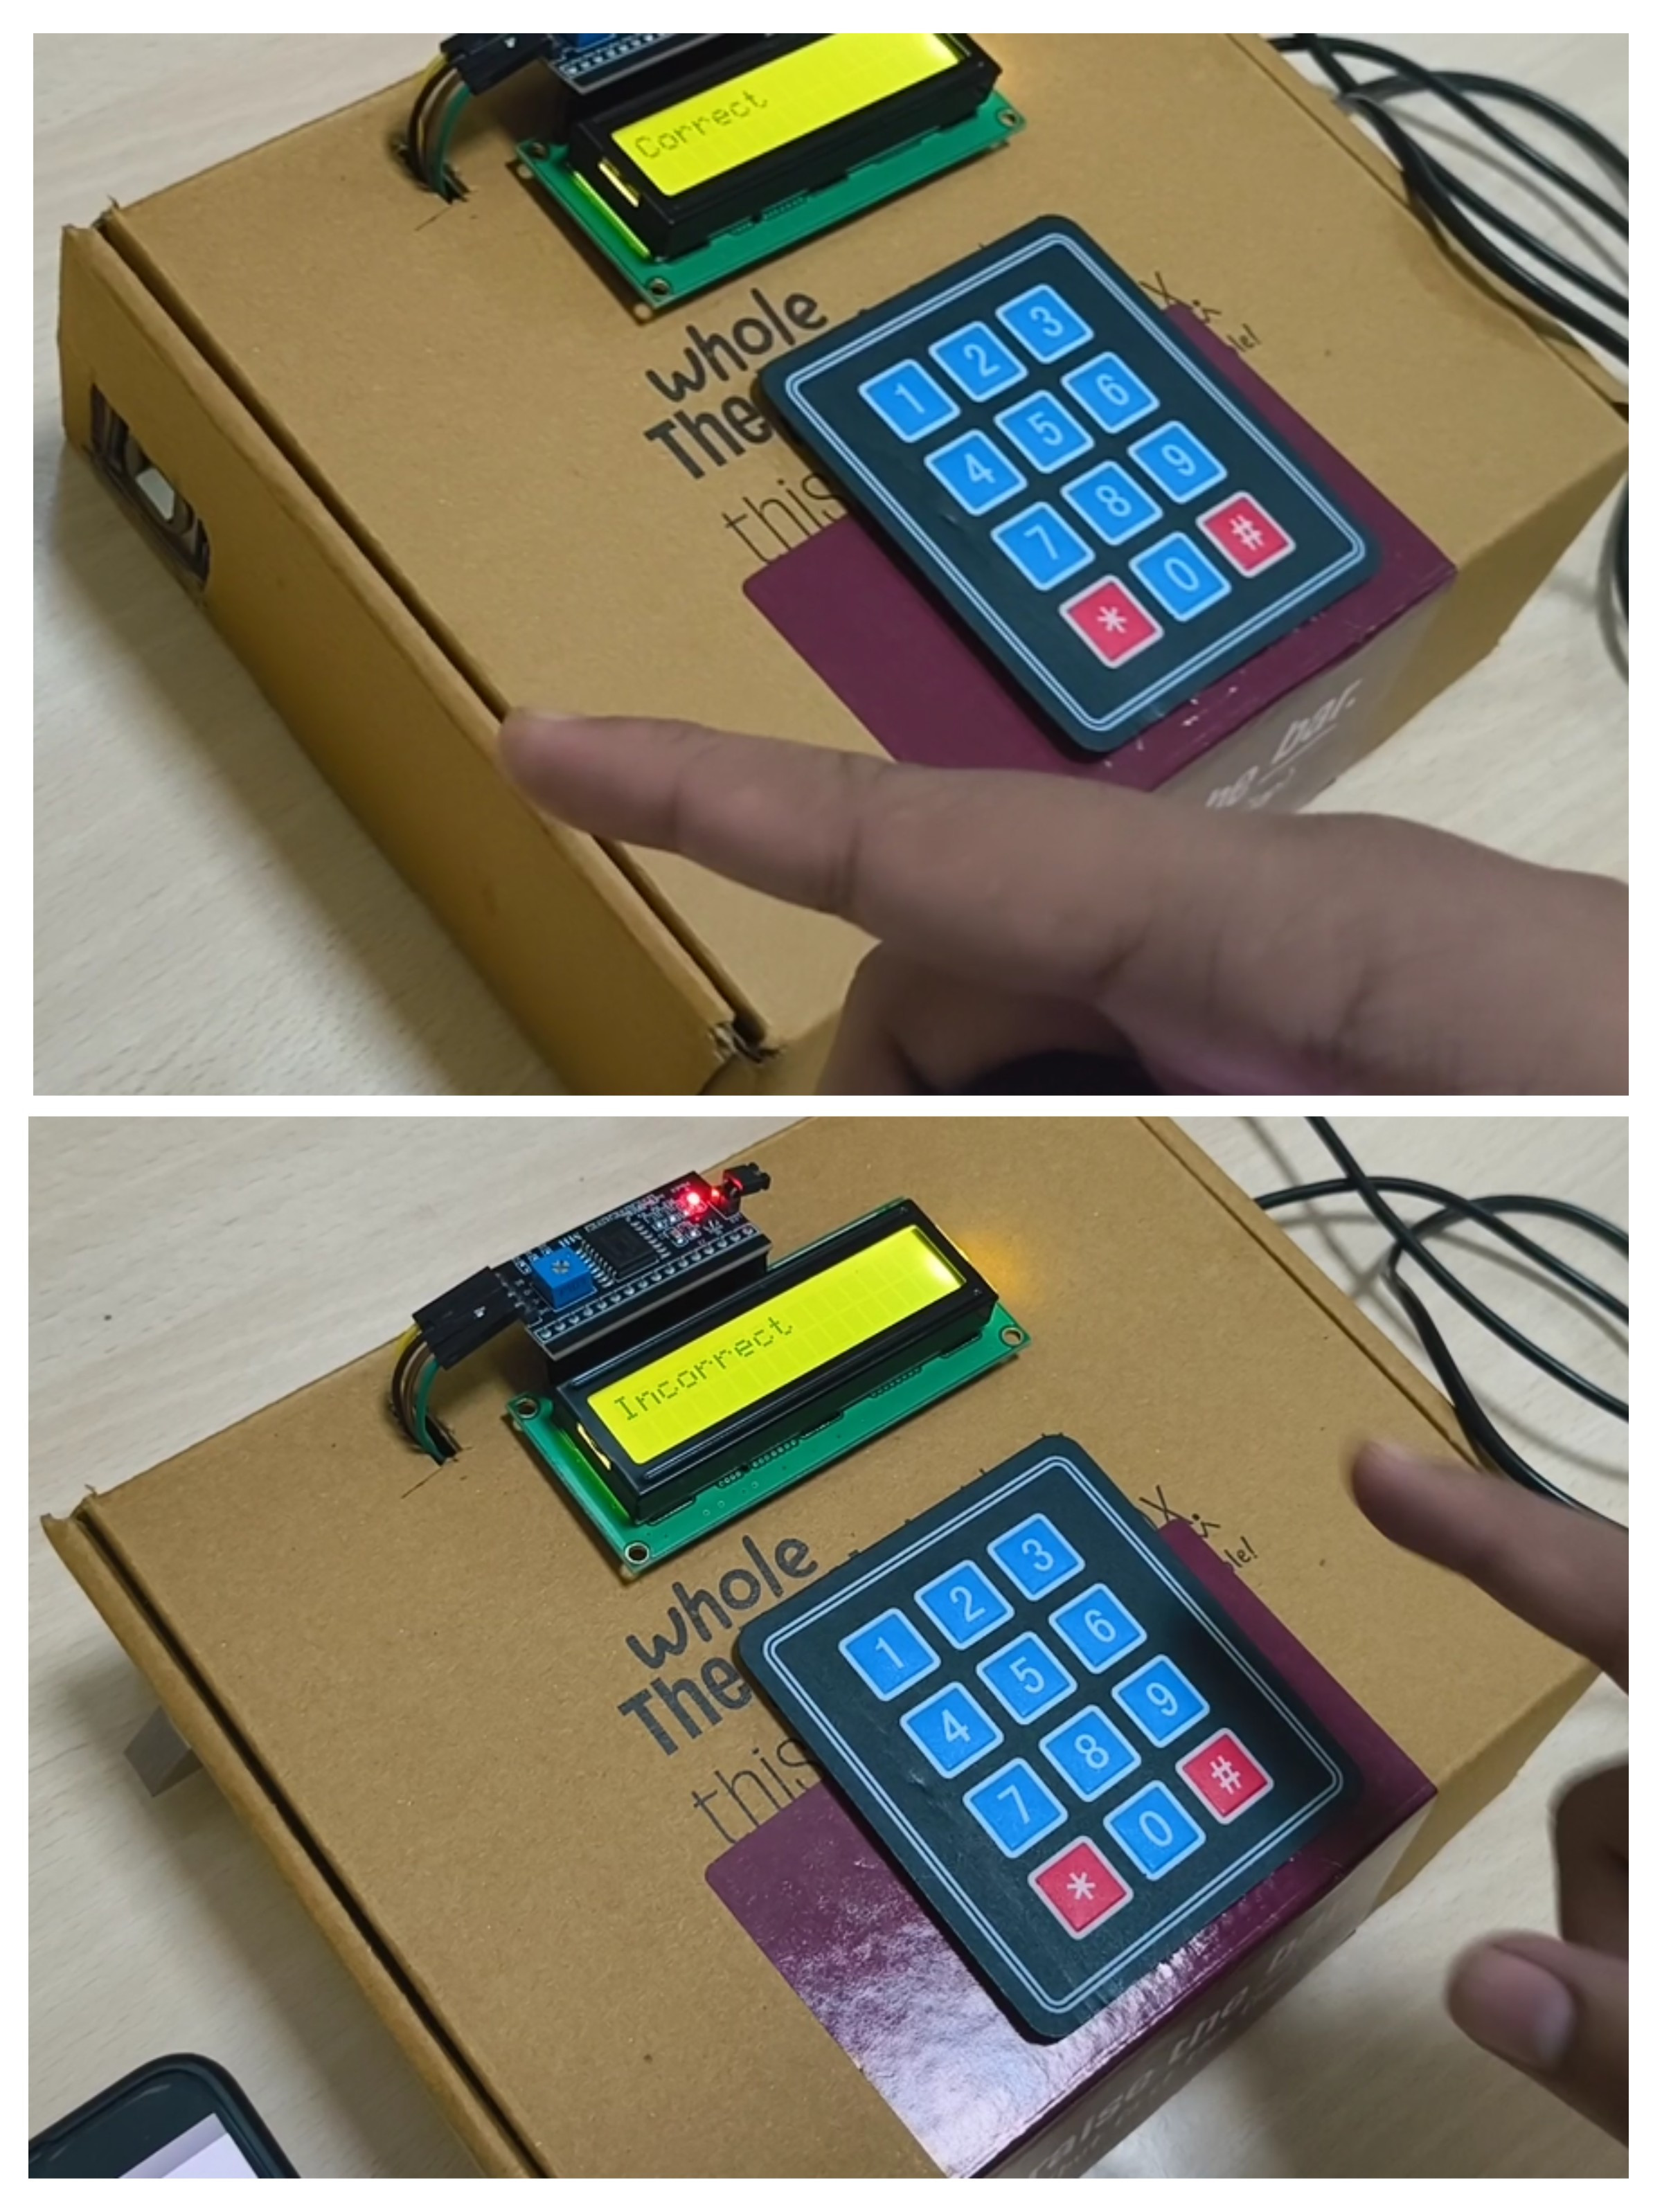
\includegraphics[width=0.8\textwidth]{20241202_032338-COLLAGE.jpg}
    \caption{Results Visualization}
\end{figure}

\section{Simulation and Short Video Demonstration}
\begin{itemize}
    \item Simulation Software: We did not find any software providing all the components we are using in the simulation hence we were unable to create a simulation. 
    \item Demonstration Video: \href{https://iiitaphyd-my.sharepoint.com/:v:/g/personal/harry_jain_research_iiit_ac_in/EdGUeO9bXKJGoRh8uWHGxhgBBLm3FiaC0rY1k3uBpZZm1g?e=NOyhcC}{link to video}
    \begin{center}
        \textbf{QR Code for the video:}
        \\
        \vspace{1em}
        \qrcode{https://iiitaphyd-my.sharepoint.com/:v:/g/personal/harry_jain_research_iiit_ac_in/EdGUeO9bXKJGoRh8uWHGxhgBBLm3FiaC0rY1k3uBpZZm1g?e=NOyhcC}
    \end{center}
\end{itemize}

\section{Photos}
\begin{figure}[H]
    \centering
    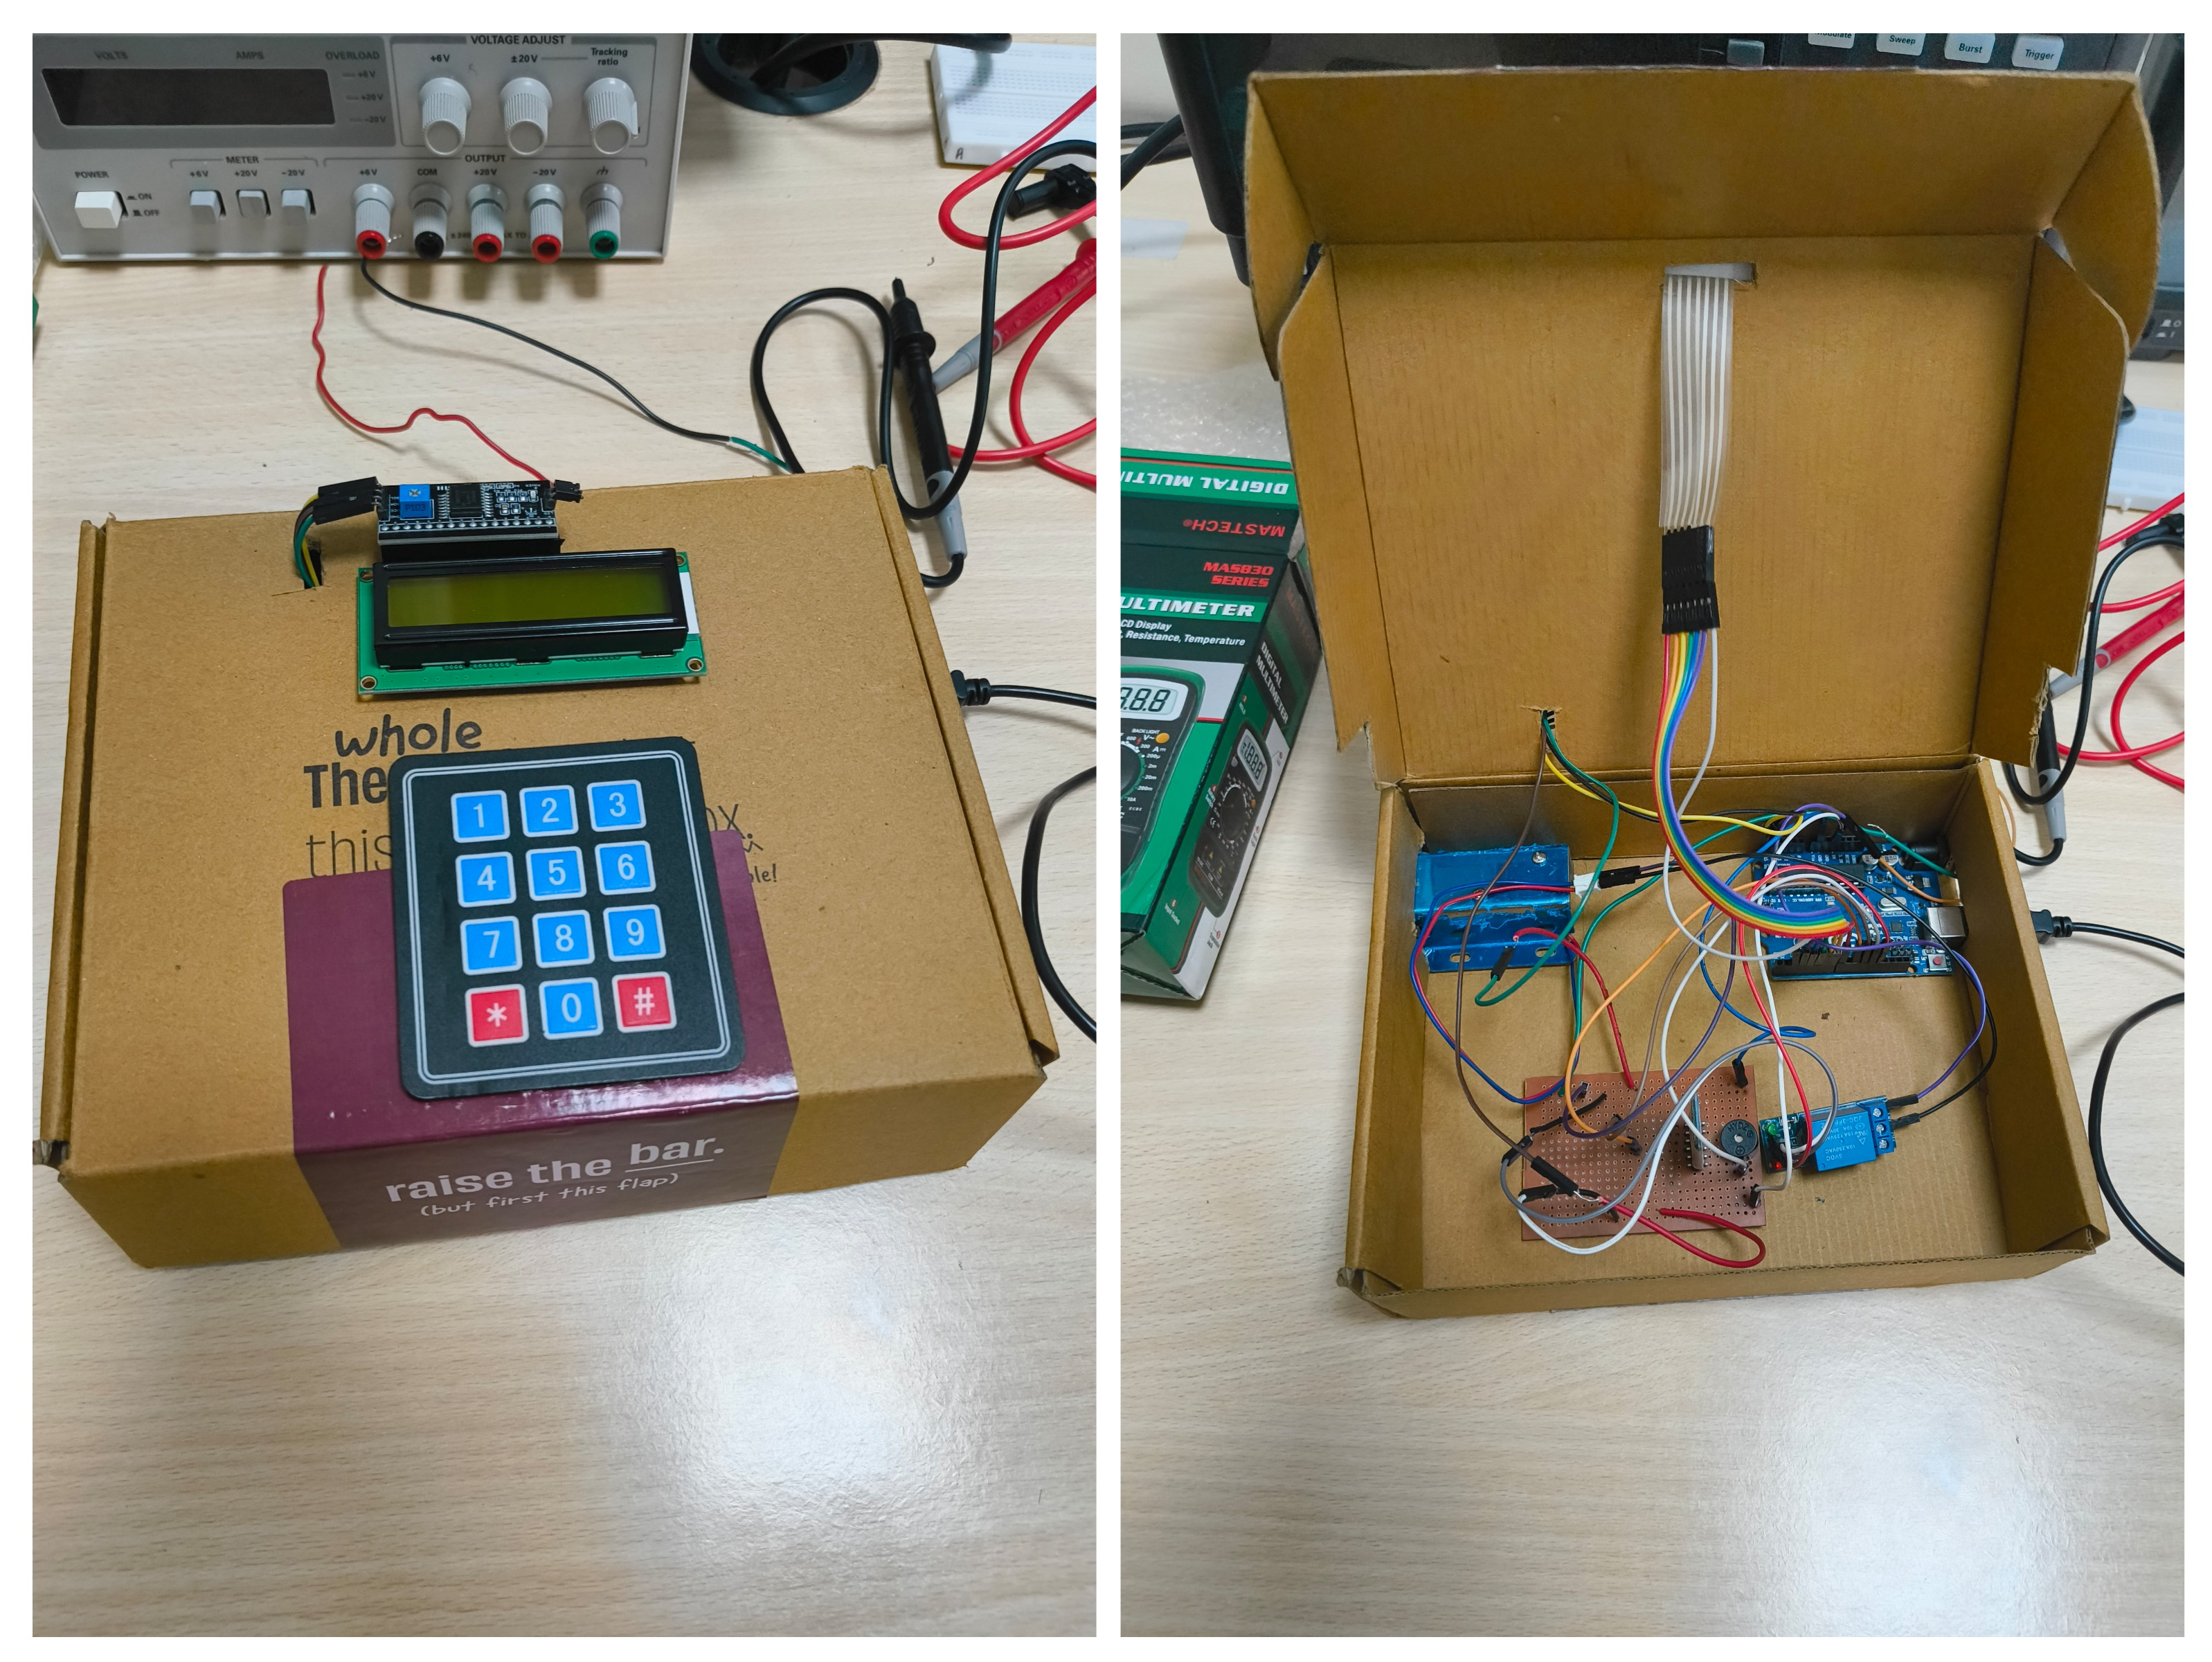
\includegraphics[width=0.8\textwidth]{20241202_025518-COLLAGE.jpg}
    \caption{Project Setup}
\end{figure}

\section{Bibliography}
\begin{thebibliography}{9}
    \bibitem{keypad}
    Arduino Official Documentation, \textit{Keypad Library for Arduino}, Available at: \url{https://www.arduino.cc/reference/en/libraries/keypad/}.
    
    \bibitem{bluetooth}
    Arduino Official Documentation, \textit{Interfacing HC-05 Bluetooth Module with Arduino}, Available at: \url{https://www.arduino.cc/en/Guide/ArduinoBT}.
    
    \bibitem{lcd}
    Arduino Official Documentation, \textit{I2C Interface for LCDs}, Available at: \url{https://projecthub.arduino.cc/arduino_uno_guy/i2c-liquid-crystal-displays-5eb615}.
    
    \bibitem{relay}
GEYA, \textit{What is a Relay Module and What Does It Do?}, Available at: \url{https://www.geya.net/what-is-a-relay-module-and-what-does-it-do/}.

    \bibitem{mitappinventor}
    MIT App Inventor Documentation, \textit{Getting Started with App Inventor}, Available at: \url{https://appinventor.mit.edu/explore/get-started}.
\end{thebibliography}

\appendix
\section{Source Code}

The following is the source code for the Arduino-based door lock system with password protection:
For 

\begin{lstlisting}[language=C,caption={Arduino Source Code for Password Protected Door Lock},label={lst:source_code},basicstyle=\small\ttfamily]
#include <Wire.h>  // Include Arduino Wire library for I2C
#include <LiquidCrystal_I2C.h>  // Include LCD display library 
                                for I2C
#include <Keypad.h>  // Include Keypad library
#include <SoftwareSerial.h>  // Include Serial library

SoftwareSerial mySerial(10, 11);  // 10 - Rx, 11 - Tx

#define Password_Length 9  // Length of password + 1 for 
                            null character

char Data[Password_Length];  // Character to hold password input
char Master[Password_Length] = "12345678";  // Password

int lockOutput = 13;  // Pin connected to lock relay input
int buzzerPin = 12;  // Pin connected to buzzer
int countinc = 0;  // counter for incorrect attempts, max att
#define MAXINC 3

byte data_count = 0;  // Counter for character entries
char btKey;  // Character to hold Bluetooth key input
char keyKey;  // Character to hold keypad key input
char customKey;  // Custom key

const byte ROWS = 4;  // Constants for row sizes
const byte COLS = 3;  // Constants for column sizes

// Array to represent keys on keypad
char hexaKeys[ROWS][COLS] = {
  { '1', '2', '3' },
  { '4', '5', '6' },
  { '7', '8', '9' },
  { '*', '0', '#' }
};

// Connections to Arduino
byte rowPins[ROWS] = { 8, 7, 6, 5 };
byte colPins[COLS] = { 4, 3, 2 };

// Create keypad object
Keypad customKeypad = Keypad(makeKeymap(hexaKeys), 
rowPins, colPins, ROWS, COLS);

// Create LCD object
LiquidCrystal_I2C lcd(0x27, 16, 2);

void setup() {
  lcd.backlight();
  lcd.init();
  pinMode(lockOutput, OUTPUT);
  pinMode(buzzerPin, OUTPUT);
  mySerial.begin(9600);
  Serial.begin(115200);
}

void loop() {
  lcd.setCursor(0, 0);
  lcd.print("Enter Password:");

  getChar();
  if (customKey) {
    if (customKey == '*') {
      showPass();
      goto shown;
    }
    if (customKey == '#') {
      backspace();
      goto shown;
    }
    Data[data_count] = customKey;
    lcd.setCursor(data_count, 1);
    lcd.print('*');
    data_count++;
  }

  if (data_count == Password_Length - 1) {
    delay(500);
    lcd.clear();

    if (!strcmp("00000000", Data)) {
      changepass();
      goto endofloop;
    }

    if (!strcmp(Data, Master)) {
      lcd.print("Correct");
      digitalWrite(buzzerPin, HIGH);
      delay(500);
      digitalWrite(buzzerPin, LOW);
      digitalWrite(lockOutput, HIGH);
      delay(5000);
      digitalWrite(lockOutput, LOW);
      digitalWrite(buzzerPin, HIGH);
      delay(100);
      digitalWrite(buzzerPin, LOW);
    } else {
      lcd.print("Incorrect");
      digitalWrite(buzzerPin, HIGH);
      delay(100);
      digitalWrite(buzzerPin, LOW);
      delay(50);
      digitalWrite(buzzerPin, HIGH);
      delay(100);
      digitalWrite(buzzerPin, LOW);

      delay(1000);
      countinc++;
      if (countinc == MAXINC) {
        lcd.clear();
        lcd.print("Too many in-");
        lcd.setCursor(0, 1);
        lcd.print("correct attempts.");
        for (int i = 0; i < 3; i++) {
          digitalWrite(buzzerPin, HIGH);
          delay(100);
          digitalWrite(buzzerPin, LOW);
          delay(50);
          digitalWrite(buzzerPin, HIGH);
          delay(100);
          digitalWrite(buzzerPin, LOW);
          delay(100);
        }
        delay(1000);
        lcd.clear();
        lcd.print("Try again later");
        digitalWrite(buzzerPin, HIGH);
        delay(1500);
        digitalWrite(buzzerPin, LOW);
        delay(3500);
        countinc = 0;
      }
    }

endofloop:
    NULL;

    lcd.clear();
    clearData();
  }

shown:
    NULL;
}

void clearData() {
  while (data_count != 0) {
    Data[data_count] = 0;
    data_count--;
  }
  return;
}

void showPass() {
  lcd.clear();
  lcd.setCursor(0, 0);
  lcd.print("Check Password:");
  lcd.setCursor(0, 1);
  for (int i = 0; i < data_count; i++) {
    lcd.print(Data[i]);
  }
  delay(1500);
  lcd.clear();
  lcd.setCursor(0, 0);
  lcd.print("Enter Password:");
  lcd.setCursor(0, 1);
  for (int i = 0; i < data_count; i++) {
    lcd.print('*');
  }
}

void backspace() {
  if (data_count) {
    data_count--;
    lcd.clear();
    lcd.print("Enter Password:");
    lcd.setCursor(0, 1);
    for (int i = 0; i < data_count; i++) {
      lcd.print('*');
    }
  }
}

void changepass() {
  clearData();
  lcd.clear();
  lcd.print("Reset Password?");
  lcd.setCursor(0, 1);
  lcd.print("Yes (1), No (0)");

  do {
    getChar();
  } while (!customKey);
  if (customKey == '1') {
    lcd.clear();
    lcd.print("Old Password:");
    for (int i = 0; i < 8; i++) {
      do {
        getChar();
      } while (!customKey);
      if (customKey) {
        if (customKey == '*') {
          showPass();
          i = i - 1;
          continue;
        }
        if (customKey == '#') {
          lcd.setCursor(0, 0);
          lcd.print("Incorrect input");
          delay(500);
          lcd.setCursor(0, 0);
          lcd.print("Old Password:  ");
          i = i - 1;
          continue;
        }
        Data[data_count] = customKey;
        lcd.setCursor(data_count, 1);
        lcd.print('*');
        data_count++;
      }
    }
    if (!strcmp(Data, Master)) {
      lcd.clear();
      lcd.print("Correct");
      delay(1000);
      lcd.clear();
      lcd.print("Enter new");
      lcd.setCursor(0, 1);
      lcd.print("Password:");
      delay(1000);
      lcd.clear();
      lcd.print("Password:");

      for (int i = 0; i < 8; ++i) {
        do {
          getChar();
        } while (!customKey);
        if (customKey) {
          if (customKey == '*') {
            lcd.setCursor(0, 0);
            lcd.print("Incorrect input");
            delay(500);
            lcd.setCursor(0, 0);
            lcd.print("Password:      ");
            i = i - 1;
            continue;
          }
          if (customKey == '#') {
            lcd.setCursor(0, 0);
            lcd.print("Incorrect input");
            delay(500);
            lcd.setCursor(0, 0);
            lcd.print("Password:      ");
            i = i - 1;
            continue;
          }
          lcd.setCursor(i, 1);
          lcd.print('*');
          Master[i] = customKey;
        }
      }
      lcd.clear();
      lcd.print("Password Reset");
      lcd.setCursor(0, 1);
      lcd.print("Complete");
      delay(500);
      digitalWrite(buzzerPin, HIGH);
      delay(500);
      digitalWrite(buzzerPin, LOW);
      delay(100);
      digitalWrite(buzzerPin, HIGH);
      delay(500);
      digitalWrite(buzzerPin, LOW);
      delay(100);
      digitalWrite(buzzerPin, HIGH);
      delay(500);
      digitalWrite(buzzerPin, LOW);
      delay(1000);
      lcd.clear();
    } else {
      lcd.clear();
      lcd.print("Incorrect");
      lcd.setCursor(0, 1);
      lcd.print("Password");
      digitalWrite(buzzerPin, HIGH);
      delay(100);
      digitalWrite(buzzerPin, LOW);
      delay(1000);
    }
    return;
  } else
    return;
}

void getChar() {
  btKey = 0;
  if (mySerial.available()) {
    btKey = mySerial.read();
  }
  keyKey = customKeypad.getKey();
  customKey = 0;
  if (btKey || keyKey) {
    customKey = keyKey ? keyKey : btKey;
  }
  if (customKey) {
    digitalWrite(buzzerPin, HIGH);
    delay(100);
    digitalWrite(buzzerPin, LOW);
    delay(100);
  }
}
\end{lstlisting}

\clearpage
\begin{center}
    \textbf{Scan the QR code below to access the full project on GitHub, including all source code and the .apk file :}
    \\
    \vspace{1em}
    \qrcode{https://github.com/JARVISONFIRE/doorlock_prototype.git}
\end{center}



\end{document}
